\documentclass[12pt]{article}    
\usepackage{ucs} 
\usepackage[utf8x]{inputenc}
\usepackage[russian]{babel}  
\usepackage{float}
\usepackage{amsmath}
\usepackage{autonum}
\title{Лабораторная работа №7\\
		Определение постоянной Планка}
\author{Хафизов Фанис}
\usepackage[pdftex]{graphicx}
\usepackage{multirow}
\begin{document}
	\begin{figure}
		\centering
		
\includegraphics[width=0.3\linewidth]{logo}
	\end{figure}
	\maketitle
	\newpage
	\section{Цель работы}
	\begin{enumerate}
		\item
		Изучение явления внешнего фотоэлектрического эффекта и проверка справедливости уравнения Эйнштейна для фотоэффекта;
		\item
		Экспериментальное определение постоянной Планка.
	\end{enumerate}
	\section{Оборудование}
	\begin{figure}[H]
		\centering
		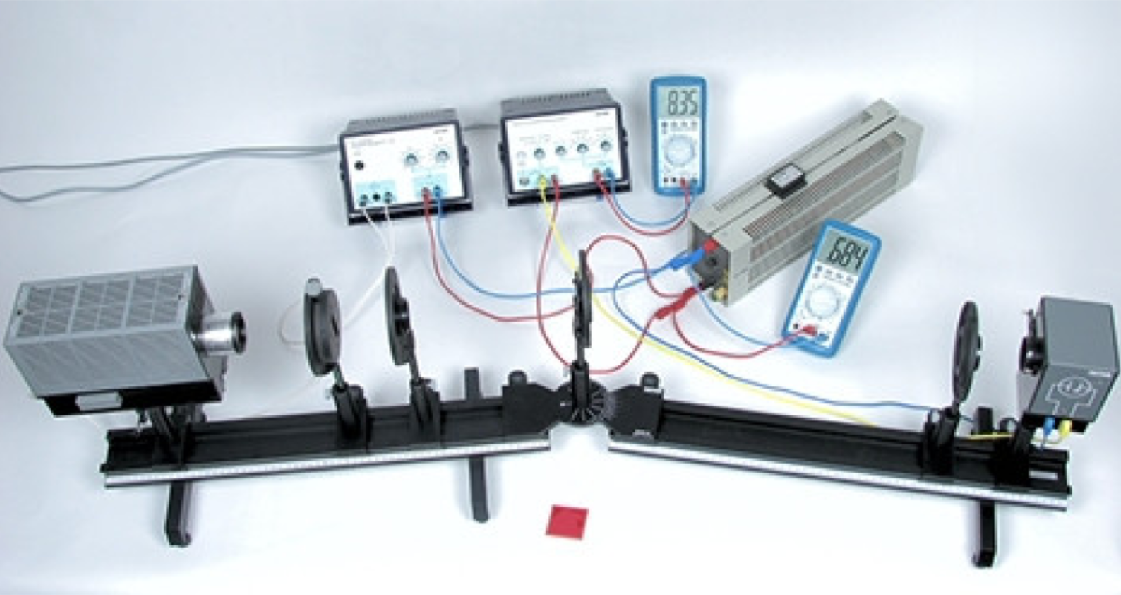
\includegraphics[width=\linewidth]{scheme}
		\caption{Экспериментальная установка для измерения фототока.}
	\end{figure}
	Эксперимент по демонстрации фотоэлектрического эффекта формируется с помощью следующих элементов: фотоэлемента, катод которого облучается лучом света, который характеризуется частотой $\nu$; потенциометра, позволяющего применять к аноду напряжение $U$ (положительное или отрицательное по отношению к катоду); вольтметра для измерения данного напряжения; микроамперметра для измерения фотоэлектрического тока $I$.
	\section{Порядок действий}
	\begin{enumerate}
		\item
		Соберем экспериментальную установку.
		\item
		Получим экспериментальную зависимость напряжения на резисторе, подключенного последовательно с фотоэлементом $U$ от угла $\varphi$ в пределах от 13$^\circ$ до 25$^\circ$. Построим график этой зависимости.
		\item
		Для фиксированного значения $\varphi=20^\circ$ получим зависимость напряжения на резисторе при фотоэлементе от приложенного напряжения между анодом и катодом $U(U_1)$. Построим график этой зависимости и по нему определим запирающее напряжение для данной длины волны излучения.
		\item
		Исследуем зависимость запирающего напряжения от длины волны излучения, определяя минимальное по модулю напряжение между анодом	и катодом, при котором прекращается фототок.
		\item
		Построим график зависимости запирающего напряжения $U_{3}$ от длины волны излучения $\lambda$ в координатах, в которых она будет линейной. По графику определим постоянную Планка. Оценим погрешность.
	\end{enumerate}
	\section{Теоретическая зависимость}
	Формула дифракционной решетки:
	\[
	m\cdot\lambda=d\cdot\sin(\varphi)
	\label{eq1:ref}
	\]
	Так как мы наблюдаем первый дифракционный максимум, то $m=1$.\\
	Уравнение Эйнштейна для фотоэффекта:
	\[
	h\frac{c}{\lambda} = A_B + e\cdot U_3
	\label{eq2:ref}
	\]
	\[
	\displaystyle
	(\ref{eq1:ref}), (\ref{eq2:ref}) \Rightarrow 
	U_3=\frac{1}{e}(\frac{hc}{d\sin(\varphi)}-A_B)
	\label{eq3:ref}
	\]
	Получили, что запирающее напряжение пропорционально $\displaystyle\frac{1}{\sin(\varphi)}$.
	\section{Таблицы данных и графики}
	\begin{table}[H]
		\centering
		\begin{tabular}{|l|l|}
			\hline
			$\varphi, ^\circ$     & $U$, В \\ \hline
			13 & 6,5    \\ \hline
			14 & 8,9    \\ \hline
			15 & 14,0   \\ \hline
			16 & 14,0   \\ \hline
			17 & 14,0   \\ \hline
			18 & 14,0   \\ \hline
			19 & 14,0   \\ \hline
			20 & 14,0   \\ \hline
			21 & 14,0   \\ \hline
			22 & 14,0   \\ \hline
			23 & 9,9    \\ \hline
			24 & 7,1    \\ \hline
			25 & 6,5    \\ \hline
		\end{tabular}
		\caption{Зависимость $U(\varphi)$}
	\end{table}
	\begin{table}[H]
		\centering
		\begin{tabular}{|r|r|}
			\hline
			\multicolumn{1}{|l|}{$U_1$, В} & \multicolumn{1}{l|}{$U$, В} \\ \hline
			7,5                            & 13,97                       \\ \hline
			7,17                           & 13,5                        \\ \hline
			7,15                           & 12,74                       \\ \hline
			7,12                           & 11,35                       \\ \hline
			7,09                           & 10,22                       \\ \hline
			7,06                           & 9,1                         \\ \hline
			7,03                           & 8,15                        \\ \hline
			7                              & 7,2                         \\ \hline
			6,97                           & 6,52                        \\ \hline
			6,92                           & 5,75                        \\ \hline
			6,89                           & 5,55                        \\ \hline
			6,82                           & 5,4                         \\ \hline
		\end{tabular}
	\caption{Зависимость $U(U_1)$}
	\end{table}
	\begin{table}[H]
		\centering
		\begin{tabular}{|l|r|l|}
			\hline
			$\varphi, ^\circ$ & \multicolumn{1}{l|}{$1/\sin(\varphi)$} & $U_1$, В \\ \hline
			15                & 3,86                                           & 6,83     \\ \hline
			16                & 3,62                                           & 6,89     \\ \hline
			17                & 3,42                                           & 7,09     \\ \hline
			18                & 3,23                                           & 7,04     \\ \hline
			19                & 3,07                                           & 7,07     \\ \hline
			20                & 2,92                                           & 7,10     \\ \hline
			21                & 2,79                                           & 7,21     \\ \hline
			22                & 2,67                                           & 7,36     \\ \hline
		\end{tabular}
		\caption{Зависимость $U_3(1/\sin(\varphi))$}
	\end{table}
	\begin{figure}[H]
		\centering
		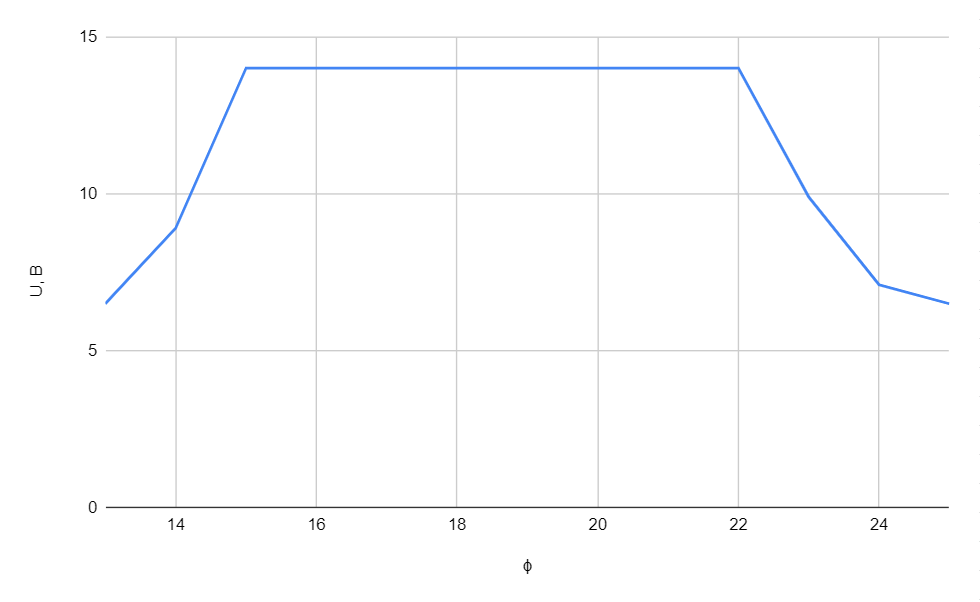
\includegraphics[width=\linewidth]{graph1}
		\caption{График зависимости $U(\varphi)$.}
	\end{figure}
	\begin{figure}[H]
		\centering
		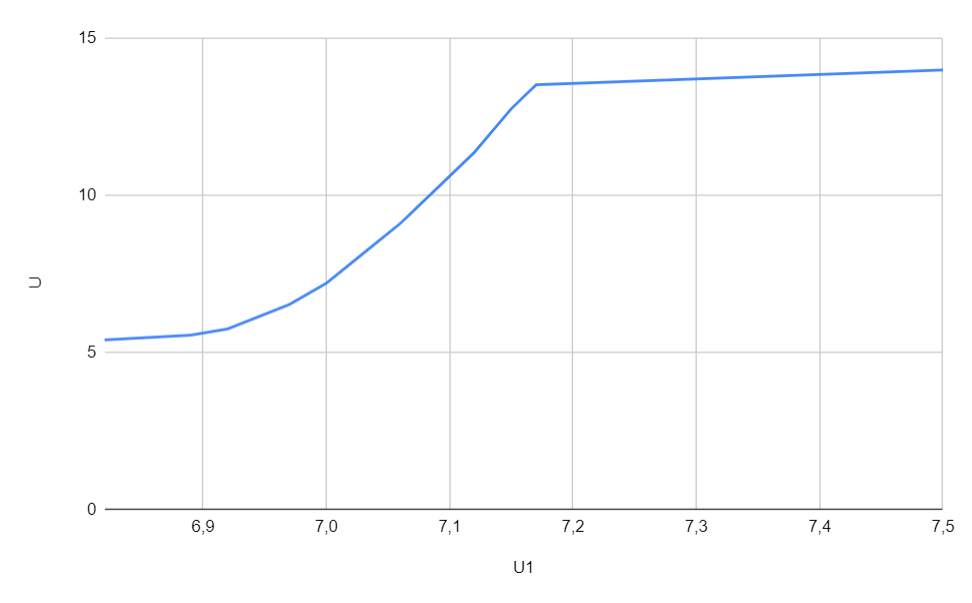
\includegraphics[width=0.9\linewidth]{graph2}
		\caption{График зависимости $U(U_1)$.}
	\end{figure}
	\begin{figure}[H]
		\centering
		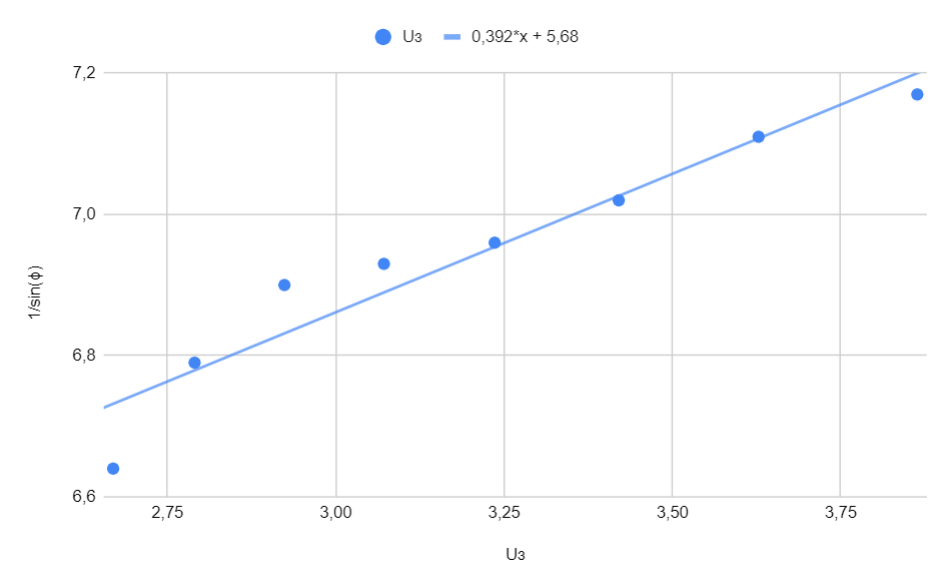
\includegraphics[width=0.9\linewidth]{graph3}
		\caption{График зависимости $U_3(1/\sin(\varphi))$.}
	\end{figure}
	\section{Расчеты}
	Угловой коэффициент графика зависимости $U_3(1/\sin(\varphi))$ равен $\alpha=0,392 B$. Из (\ref{eq3:ref}) $\displaystyle\alpha=\frac{hc}{ed}$.\\
	$
	\displaystyle
	h=\frac{\alpha ed}{c} = \frac{0,392\cdot 1,6 \cdot 10^{-19} \cdot 1,67 \cdot 10^{-6}}{3\cdot 10^8}=3,49\cdot 10^{-34} 
	$ Дж$\cdot$с\\
	$\displaystyle \Delta h=h\cdot \varepsilon_h=h\cdot\varepsilon_\alpha=h(\varepsilon_{U_3} + \varepsilon_{\sin\alpha})=h(\frac{\Delta{U_3}}{U_3} + \frac{\cos\alpha \Delta\alpha}{\sin\alpha})=3,49\cdot 10^{-34}(\frac{0,02}{6,64}+0,07)=0,26\cdot10^{-34}$Дж$\cdot$с\\
	$\varepsilon_h=\frac{\Delta h}{h}=7,5\%$\\
	$h = (3,49\pm0,26)10^{-34}$Дж$\cdot$с
	\section{Выводы}
	Экпериментально полученное значение постоянной Планка значительно отличается от табличных данных (примерно в 2 раза), но порядок значений совпадает. Причиной этого могла стать погрешность, связанная с оборудованием. Из-за этого вычисленная погрешность является небольшой, хотя расхождение в жизни велико.
\end{document}